              %%%%%%%%%%%%%%%%%%%%%%%%%%%%%%%%%%%%%%%%%%%%%%%%%%%%%%%%%%%%%%%%%%%%%%%%%%%%%%%
%%% SWEAVE
       % Ihaka, R. (2009). Customizing Sweave 
%%%%%%%%%%%%%%%%%%%%%%%%%%%%%%%%%%%%%%%%%%%%%%%%%%%%%%%%%%%%%%%%%%%%%%%%%%%%%%%
%%% CUSTOMIZING SWEAVE 
%%% from: Ihaka, R. (2009). Customizing Sweave to Produce Better Looking LATEX Output
\DefineVerbatimEnvironment{Sinput}{Verbatim}{fontsize=\footnotesize, formatcom=\color{codecolor}, xleftmargin=2em}
\DefineVerbatimEnvironment{Soutput}{Verbatim}{fontsize=\footnotesize, xleftmargin=2em, formatcom=\color{codecolor}} 
\DefineVerbatimEnvironment{Scode}{Verbatim}{fontsize=\footnotesize, xleftmargin=2em, formatcom=\color{codecolor}}

\renewenvironment{Schunk}{\vspace{10pt}}{\vspace{8pt}}   
%%%%%%%%%%%%%%%%%%%%%%%%%%%%%%%%%%%%%%%%%%%%%%%%%%%%%%%%%%%%%%%%%%%%%%%%%%%%%%%
%%%%%%%%%%%%%%%%%%%%%%%%%%%%%%%%%%%%%%%%%%%%%%%%%%%%%%%%%%%%%%%%%%%%%%%%%%%%%%%

\section{Formel für Konfidenzintervalle für binomiale Anteile überprüfen}

Nehmen wir haben in einer Umfrage mit $n=500$ Personen erfragt, ob sie die FDP wählen würden, wenn kommenden Sonntag Bundestagswahl wäre. $5\%$ der Befragten gaben an, dass sie die Partei wählen würden. Wie groß ist das Konfidenzinterval? In vielen Statistikehrbüchern wird folgenden Formel für die Berechnung der Konfidenzintervalle für binomiale Anteilswerte aufgeführt. 

\begin{equation} \label{eq:prop_standard}
\hat p + z_{1- \frac{\alpha}{2}} \cdot \frac{\sqrt{\hat p(1-\hat p)}}{\sqrt{n}}
\end{equation}

% \begin{eqnarray} \label{eq:prop_standard_2}
% c = \Phi^{-1} \left( 1 - {\alpha \over 2} \right) \\
% p_u = \hat p - c \cdot \sqrt{\hat p \cdot (1-\hat p) \over n} \\
% p_o = \hat p + c \cdot \sqrt{\hat p \cdot (1-\hat p) \over n} 
% \end{eqnarray}   
  
Schreiben wir hierzu in \R{} eine Funktion, die dies berechnet.

\begin{Schunk}
\begin{Sinput}
> ci_standard <- function(p.hat, n, alpha=.05){
   ci <- qnorm(1 - alpha/2) * sqrt(p.hat * (1 - p.hat) / n) 
   lower <- p.hat - ci                       # oberes KI            
   upper <- p.hat + ci                       # unteres KI
   c(p.hat=p.hat, lower=lower, upper=upper)
 }  
> ci_standard(p.hat=.05, n=500)
\end{Sinput}
\begin{Soutput}
     p.hat      lower      upper 
0.05000000 0.03089663 0.06910337 
\end{Soutput}
\end{Schunk}

Gemäß der Formel beläuft sich das Konfidenzintervall somit auf $0.05 \pm 0.05$. 

Es soll nun in einer Simulation überprüft werden, ob die Formel korrekte Konfidenzintervalle berechnet. Hierzu stellen wir folgende Überlegung an. Wenn wir den wahren Anteilswert $p$ in der Population kennen, können wir eine Stichprobe ziehen und schauen, ob das mittels der Formel berechnete Konfidenzintervall den wahren Wert $p$ überdeckt. Wenn wir diesen Vorgang viele Male wiederholen, so sollte das Konfidenzintervall den Wert $p$ in $(1 - \alpha) \cdot 100\,\%$ der Fälle umfassen. Hierfür wird in der Literatur der Begriff \emph{Überdeckungswahrscheinlichkeit} genutzt. Diese sollte bei für alle $p$ exakt bei $95\%$ liegen. Um zu überprüfen, ob dies der Fall ist, programmieren wir zunächst eine Funktion, die \emph{eine} Stichprobenziehung simuliert.


\begin{Schunk}
\begin{Sinput}
> sim_one_ci <- function(n, p, alpha=.05){
   vals <- rbinom(n, 1, p)                # Stichprobe ziehen 
   p.hat <- mean(vals)                    # geschätzter Anteil 
   cis <- ci_standard(p.hat, n, alpha)    # KI berechnen
   lower <- cis[["lower"]]                # unteres KI
   upper <- cis[["upper"]]                # oberes KI
   c(p.hat=p.hat,                         # Punktschätzung
     lower=lower, upper=upper,            # KIs ausgeben
     covered= lower <= p && p <= upper)   # liegt p im Intervall?
 }
> sim_one_ci(n=100, p=.1, alpha=.05)
\end{Sinput}
\begin{Soutput}
     p.hat      lower      upper    covered 
0.06000000 0.01345343 0.10654657 1.00000000 
\end{Soutput}
\end{Schunk}

Führen wir nun im Folgenden diese Ziehung mehrfach durch, um zu schauen, ob das Konfidenzintervall richtig berechnet wird. Auch hierzu schreiben wir erneut eine Funktion.

\begin{Schunk}
\begin{Sinput}
> sim_many_ci <- function(reps, n, p, alpha=.05){
   ncovered <- 0                       # Zähler p innerhalb des KI?
   for (i in 1:reps){                  # reps Male durchlaufen
     sam <- sim_one_ci(n, p, alpha)    # eine Stichprobe ziehen
     if (sam["covered"] == 1)          # ist p im Intervall?       
       ncovered <- ncovered + 1        # wenn ja Zähler erhöhen 
   }
   c(p=p, n=n,                         # Parameter zurückgeben
     prop.covered=ncovered/reps)       # Anteil p innerhalb KI
 }
\end{Sinput}
\end{Schunk}

Simulieren wir nun $1000$ Ziehungen mit einem Stichprobenumfang von $n=100$ und einem Anteilswert von $p=.05$.
 
\begin{Schunk}
\begin{Sinput}
> sim_many_ci(reps=1000, n=100, p=.1)  
\end{Sinput}
\begin{Soutput}
           p            n prop.covered 
        0.10       100.00         0.93 
\end{Soutput}
\end{Schunk}

Das Ergebnis ist überraschend. In knapp $93\,\%$ der Ziehungen liegt der $p$-Wert  innerhalb des Konfidenzintervalls. Dies ist weniger, als die erwarteten $95\,\%$. Um ausszuschließen, dass es sich hierbei um einen Stichprobenfehler handelt wiederholen wir die Simulation mit mehr Ziehungen.

\begin{Schunk}
\begin{Sinput}
> sim_many_ci(reps=10000, n=100, p=.1)  
\end{Sinput}
\begin{Soutput}
           p            n prop.covered 
      0.1000     100.0000       0.9289 
\end{Soutput}
\end{Schunk}

Das Ergebnis ändert sich kaum. Wenn wir bei der Berechnung keinen Fehler gemacht haben, so scheint die Formel also das falsche Ergebnis zu liefern. Wir entschließen uns dies näher zu explorieren und führen die Simulation mit einem anderen Anteilswert durch.

\begin{Schunk}
\begin{Sinput}
> sim_many_ci(reps=10000, n=100, p=.05)  
\end{Sinput}
\begin{Soutput}
           p            n prop.covered 
      0.0500     100.0000       0.8776 
\end{Soutput}
\end{Schunk}

Hier sind sogar noch deutlicher Abweichnungen von den $95\,\%$ zu erkennen. Um zu untersuchen, ob der Anteilswert $p$ einen Einfluss auf die Größe der Abweichung hat, führen wir eine weitere Simulation mit verschieden $p$ Werten durch.

\begin{Schunk}
\begin{Sinput}
> p_study <- function(reps, n, alpha=.05,
                     p.start=.01, p.end=.99, p.step=.1){  
   ps <- seq(p.start, p.end, p.step)                   
   rmat <- matrix(0, nrow=length(ps), ncol=3)    # Ergebnismatrix
   for (i in 1:length(ps)){                      # Durchlauf für jedes p
     p <- ps[i]                                  # neuer p Wert
     rmat[i, ] <- sim_many_ci(reps, n, p, alpha) # Ziehungen simulieren 
   } 
   res <- as.data.frame(rmat)                   
   names(res) <- c("p", "n", "prop.covered")     # Spalten benennen 
   res
 } 
\end{Sinput}
\end{Schunk}

Stellen wir die Ergebnisse nun in einer Grafik dar. Es zeigt sich, dass die Genauigkeit der berechneten Konfidenzintervalle stark von dem Anteilswert $p$ abhängt. Speziell für kleine und großer Anteilswerte scheint die Formel ungenau zu sein. 

\begin{Schunk}
\begin{Sinput}
> x <- p_study(100, 100, .05, p.step=.005)
> plot(x[c("p","prop.covered")], type="l") 
> abline(h=.95, col="red")
\end{Sinput}
\end{Schunk}
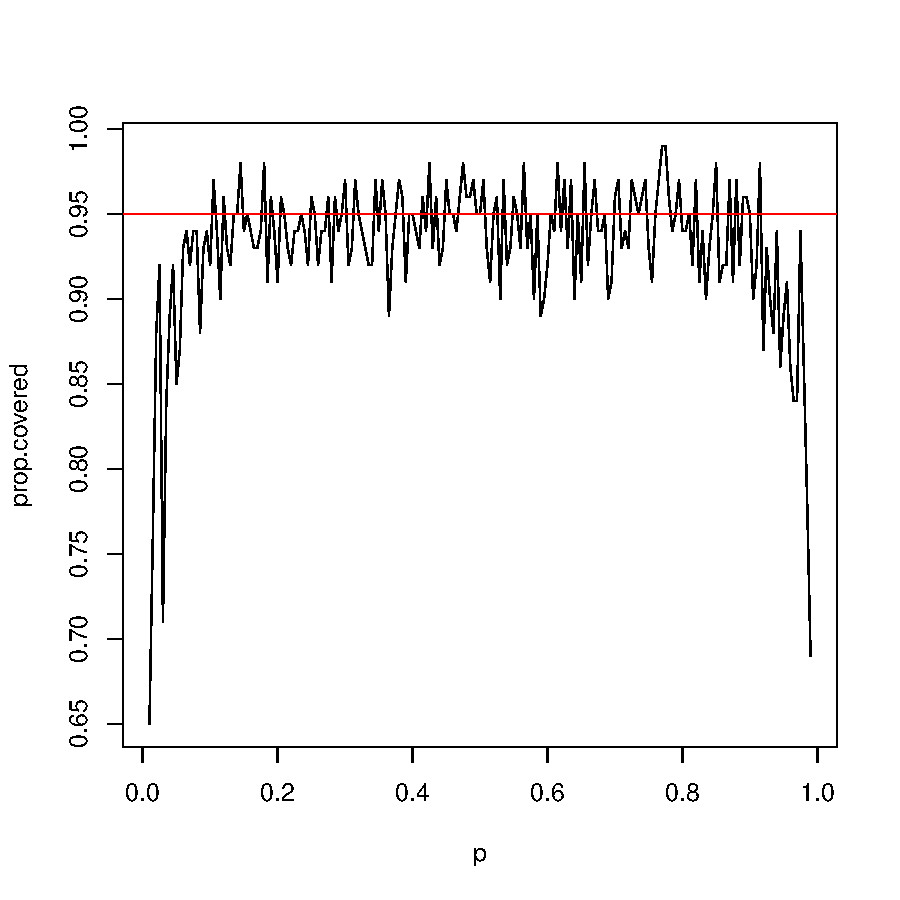
\includegraphics{sim_binomial_prop-010}

Die Frage, die sich hieran anschließt, ist ob sich neben der groben umgekehrten U-Form-Struktur weitere systematische Strukturen in der Verteilung verbergen. Hierzu wird eine erneute Analyse mit einer erhöhten Replikationszahl durchgeführt. 
 
\begin{Schunk}
\begin{Sinput}
> x <- p_study(100000, 100, .05, p.step=.005) 
> plot(x[c("p","prop.covered")], type="l") 
> abline(h=.95, col="red")
\end{Sinput}
\end{Schunk}
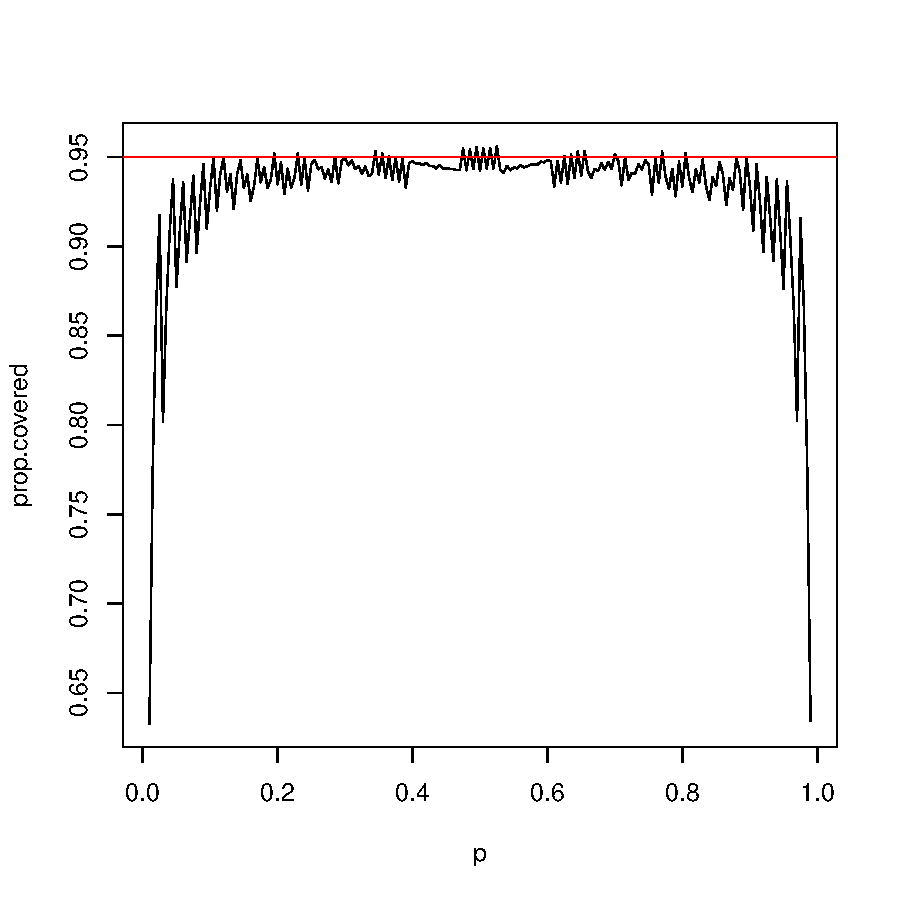
\includegraphics{sim_binomial_prop-013}

Es zeigt sich ein interessanter Effekt. Die Oszillationen der geschätzten Konfidenzintervalle in obiger Grafik ist keine Folge der geringen Replikationszahl sondern eine systematische Struktur.

Was lernen wir hieraus? Die Formel, die in viele Statistikbüchern enthalten ist, ist mit Vorsicht zu genießen, besonders bei Anteilswerten nahe $0$ oder $1$. Es gibt eine Reihe von Formeln mit besseren Eigenschaften, die später untersucht werden. Zum anderen zeigt sich eine spannende systematische Oszillation der geschätzeten Konfidenzintervalle, die wir auch bei anderen Schätzverfahren wiederfinden werden.

\textbf{Programmierung mittels Funktionen der \texttt{apply}-Familie}  

Als letzten Schritt soll demonstiert werden, wie der Code alternativ hätte geschrieben werden können. Hierzu nutzen wir anstelle von Schleifen Funktionen aus der \texttt{apply}-Familie. Der Code wird hierdurch i.d.R. kürzer. Auch führt die Nutzung von Funktionen aus der \texttt{apply}-Familie anstelle von Schleifen häufig zu einem Performancegewinn. Der Nachteil ist jedoch, dass sie am Anfang schwerer zu verstehen sind als Schleifen.
 
\begin{Schunk}
\begin{Sinput}
> sim_many_ci_2 <- function(reps, n, p, alpha=.05){
   res <- replicate(reps, sim_one_ci(n, p, alpha))
   prop.covered <- mean(res["covered", ])
   c(p=p, n=n, prop.covered=prop.covered)                   
 } 
> p_study_2 <- function(reps, n, alpha=.05,
                       p.start=.01, p.end=.99, p.step=.1){
   ps <- seq(p.start, p.end, p.step)                     
   res <- mapply(sim_many_ci_2, reps=reps,
                 n=n, p=ps, alpha=alpha)   
   as.data.frame(t(res))
 }   
> 
\end{Sinput}
\end{Schunk}

\par
\textbf{Erweiterung auf mehrere Formeln zur Schätzung der Konfidenzintervalle}  

Aufgrund der Probleme von Formel \ref{eq:prop_standard} sind in der Literatur weitere Ansätze zur Schätzung der Konfidenzintervalle für binomiale Anteile vorgeschlagen worden. Ein früher Ansatz stammt von Wilson (1927). Er schlägt folgende Intervalle vor. 

\begin{equation}  \label{eq:ci_wilson}
  p_{o,u} = \frac{1}{1 + \frac{c^2}{n}} \cdot \left(\hat p + \frac{c^2}{2n} \pm c\cdot\sqrt{\frac{\hat p \cdot (1-\hat p)}{n}+\frac{c^2}{4n^2}} \, \right)  
\end{equation}

Setzen wir diese Formel zunächst in eine \R{}-Funktion um.

\begin{Schunk}
\begin{Sinput}
> ci_wilson <- function(p.hat, n, alpha=.05){
   c <- qnorm(1 - alpha/2)
   pm <- c* sqrt(p.hat * (1 - p.hat)/n + c^2/(4*n^2))   
   c(p.hat= p.hat,
     lower= 1 / (1 + c^2/n) * (p.hat + c^2/(2*n) - pm),
     upper= 1 / (1 + c^2/n) * (p.hat + c^2/(2*n) + pm))
 } 
> ci_wilson(p.hat=.05, n=500)
\end{Sinput}
\begin{Soutput}
     p.hat      lower      upper 
0.05000000 0.03409375 0.07276816 
\end{Soutput}
\end{Schunk}

Wir wollen nun obige Analyse mit dem Wilson-Intervall wiederholen. Da wir dies zu Beginn nicht bedeacht haben, dass es mehrere Schätzverfahren gibt, sind wir gezwungen unseren Code umzuschreiben, um verschiedene Varianten einbeziehen zu können. Zur Programmierung gehen wir von der Überlegung aus, dass die Parameter die an die Funktionen übergeben werden stets $n$, $p.hat$ und $alpha$ sein werden. Wir schreiben nun eine Funktion, die das Argument \texttt{method} enthält. Über dieses kann das gewünschte Verfahren ausgewählt werden. Die Funktion match.arg sorgt hierbei dafür, dass es auch möglich ist, den Namen der Methode teilweise auszuschreiben. Wenn diese zeile weggelassen wird, müsste die Methode stets exakt benannt werden.

\begin{Schunk}
\begin{Sinput}
> ci <- function(p.hat, n, alpha=.05, method="standard"){
   method <- match.arg(method, c("standard", "wilson"))  
   if (method == "standard")
     res <- ci_standard(p.hat, n, alpha)
   if (method == "wilson")       
     res <- ci_wilson(p.hat, n, alpha)
   res
 }   
\end{Sinput}
\end{Schunk}

Erweitern wir nun unsere vorherigen Funktionen auch um das Argument \texttt{method} und ersetzen die Funktionen zur Berechnung der Konfidenzintervalle mit der Funktion \texttt{ci}.

\begin{Schunk}
\begin{Sinput}
> sim_one_ci <- function(n, p, alpha=.05, 
                         method="standard"){
   vals <- rbinom(n, 1, p)                # Stichprobe ziehen 
   p.hat <- mean(vals)                    # geschätzter Anteil 
   cis <- ci(p.hat, n, alpha, method)     # KI berechnen
   lower <- cis[["lower"]]                # unteres KI
   upper <- cis[["upper"]]                # oberes KI  
   c(p.hat=p.hat,                         # Punktschätzung
     lower= lower, upper= upper,          # KI ausgeben   
     covered= lower <= p && p <= upper)   # liegt p im Intervall?
 }
> sim_many_ci <- function(reps, n, p, alpha=.05,
                           method="standard"){
   res <- replicate(reps, sim_one_ci(n, p, alpha, method))
   prop.covered <- mean(res["covered", ])
   c(p=p, n=n, prop.covered=prop.covered)                   
 } 
> p_study <- function(reps, n, alpha=.05, method="standard",
                       p.start=.01, p.end=.99, p.step=.1){
   method <- match.arg(method, c("standard", "wilson"))  
   ps <- seq(p.start, p.end, p.step)                     
   res <- mapply(sim_many_ci, reps=reps,
                 n=n, p=ps, alpha=alpha, method=method)   
   df <- as.data.frame(t(res))
   df$method <- method
   df
 } 
\end{Sinput}
\end{Schunk}
 
Nun können wir obige Analyse für zwei Schätzverfahren durchführen. Ergänzen wir die Untersuchung nun um das Wilson-Intervall, diesmal direkt mir einer großen Replikationszahl.

\begin{Schunk}
\begin{Sinput}
> x <- p_study(100000, 100, .05, p.step=.01, method="wilson")
> plot(x[c("p","prop.covered")], type="l", las=1) 
> abline(h=.95, col="red")
\end{Sinput}
\end{Schunk}


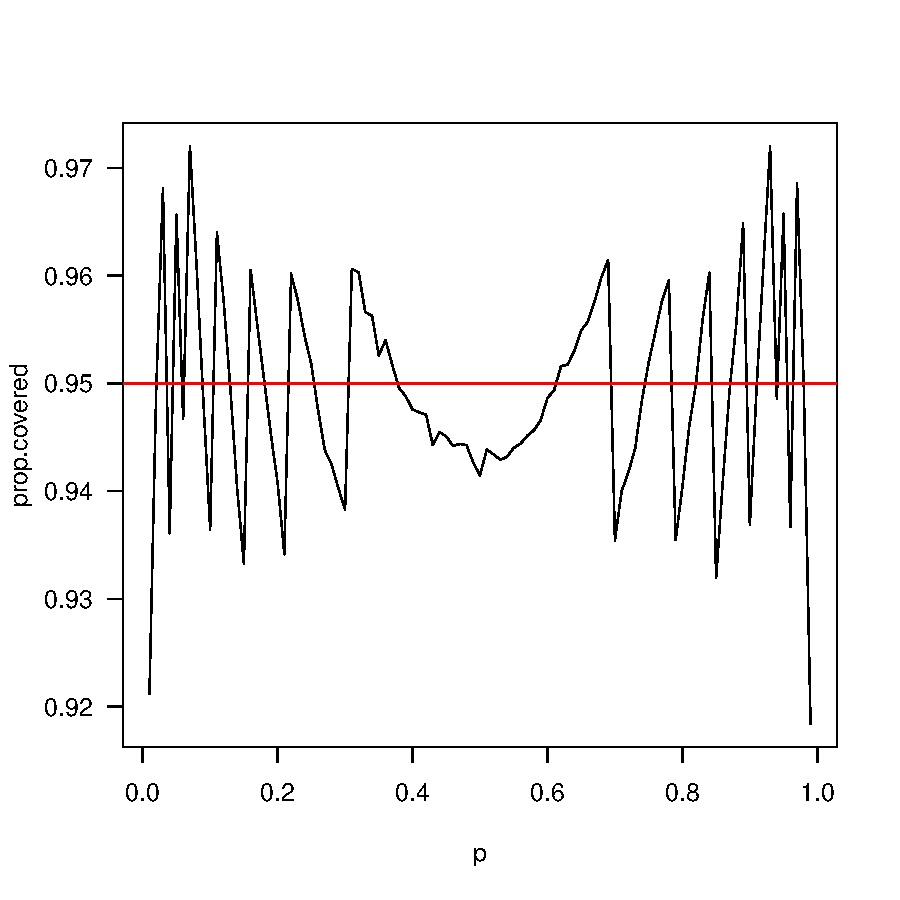
\includegraphics{sim_binomial_prop-020}

Es zeigt sich, dass die Werte deutlich dichter um $95\%$ schwanken, als bei der Standardvariante. Jedoch sind auch diese Ergebnisse keinesfalls befriedigend. Es existieren weitere Varianten, z.\,B. im Paket \texttt{binom}, die bessere Ergebnisse liefern.


\textbf{Untersuchung weiterer Parameter} 

Bisher haben wir das Verhalten des Konfidenzintervalls lediglich durch die Variation von $p$ untersucht. Die zweite Variable innerhalb der Gleichung ist $n$. Im Folgenden soll die Simulation für verschiedene $n$ und $p$ durchgeführt werden. Hierzu wird eine leere Liste angelegt, in der die Ergebnisse für jedes $n$ gespeichert werden. Die letzte Zeile verbindet die Dataframes aus den einzelnen Listenelementen zu einem großen Dataframe.

\begin{Schunk}
\begin{Sinput}
> res <- list()
> ns <- 10:100
> for (i in seq_along(ns)){
   cat(paste("\r", "run", i, "of", length(ns)))
   res[[i]] <- p_study(reps=10, n=ns[i], p.step=.1, 
                       method="standard")
 } 
> x <- do.call(rbind, res)
\end{Sinput}
\end{Schunk}

% <<eval=F>>=   
% write.csv2(x, file="data/p_study_standard_05_n100_reps1000.csv")
% @   
    

Um die Daten zu visualisieren wird die Funktion \texttt{levelplot} aus dem \texttt{lattice} Paket genutzt.
  
\begin{Schunk}
\begin{Sinput}
> library(lattice)
> levelplot(prop.covered ~ n * p, data=x)
\end{Sinput}
\end{Schunk}

Diese Visualisierung ist verbesserungsbedürftig. Uns interessiert besonders der Bereich einer Überdeckungswahrscheinlichkeit zwischen $.8$ und $1.0$. Weiterhin sollen Werte über $.95$ grüne und unterhalb rote Farben ausfweisen. Zum Erzeugen einer Farbpalette wird die Funktion \texttt{colorpanel} aus dem Paket \texttt{qplot} genutzt. 

\begin{Schunk}
\begin{Sinput}
> library(gplots)
> library(lattice) 
> levels <- seq(.8, 1, by=.05)
> colors <- c(colorpanel(4, "darkred", "red"), "lightgreen")
> levelplot(prop.covered ~ n * p, data=x, 
            at=levels, col.regions=colors)            
\end{Sinput}
\end{Schunk}
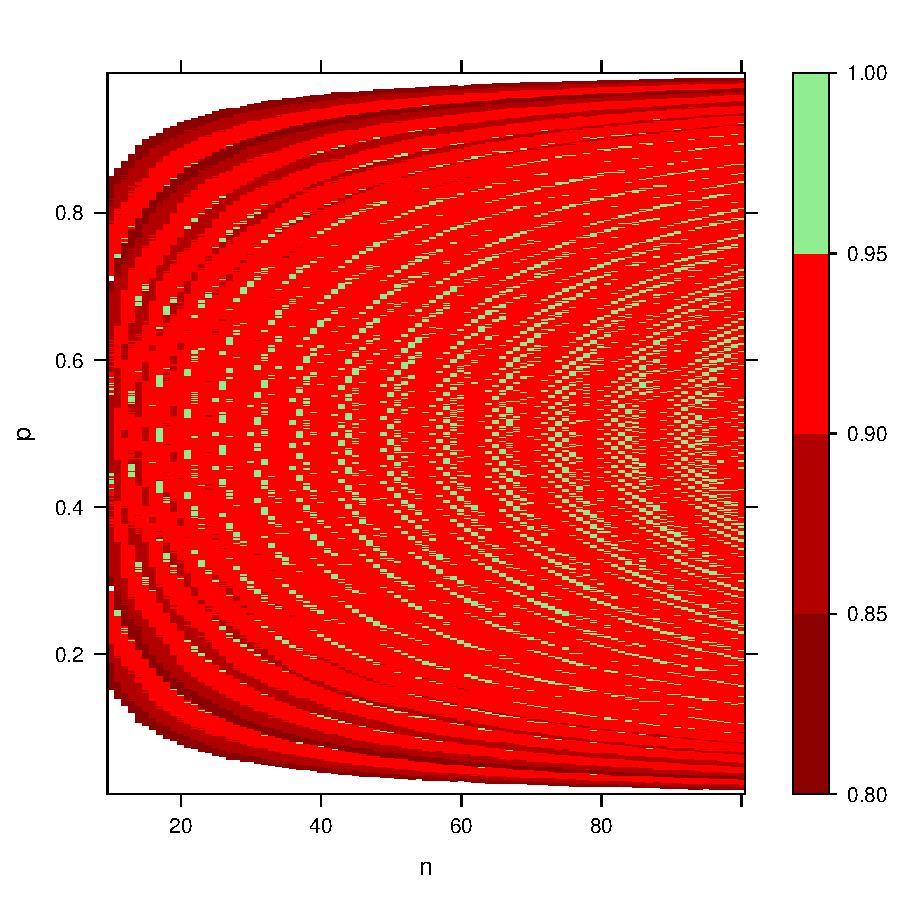
\includegraphics{sim_binomial_prop-024}

Die Grafik zeigt, dass die Performance der Formel mit steigendem $n$ in den Randbereichen von $p$ besser wird. Das oszillierende Muster bleibt jedoch auch bei größerem $n$ erhalten.


\begin{Schunk}
\begin{Sinput}
> levels <- seq(.8, 1, by=.05)
> colors <- c(colorpanel(4, "darkred", "red"), "lightgreen")
> levelplot(prop.covered ~ n * p, data=x, 
            at=levels, col.regions=colors)            
\end{Sinput}
\end{Schunk}
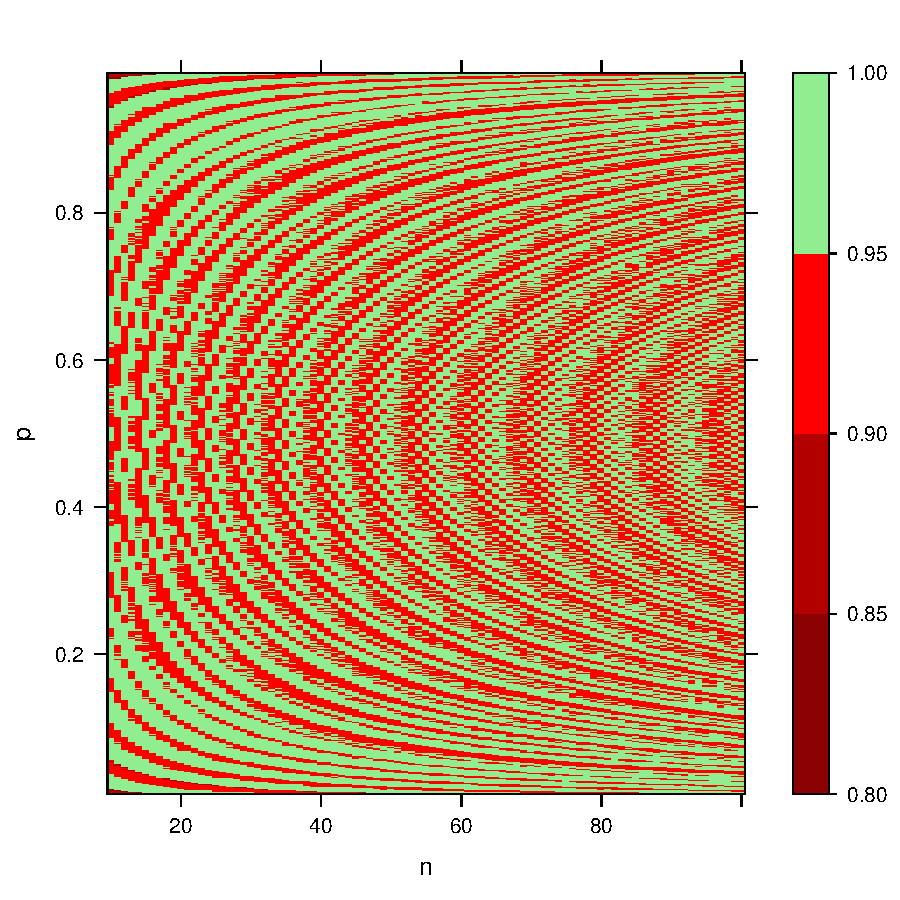
\includegraphics{sim_binomial_prop-026}

% <<>>=
% contourplot(prop.covered ~ n * p, data=x, 
%            at=levels, labels=F, region=T, col.regions=colors)
% @ 
% <<eval=F, echo=F>>=
% # alternative code
% library(gplots)
% library(reshape2)
% y <- acast(x, n ~ p, value.var="prop.covered")
% levels <- seq(.8, 1, by=.01)
% greens <- colorpanel(6, "darkgreen", "lightgreen")
% reds <- colorpanel(15, "darkred", "red")
% colors <- c(reds, greens)
% labels <- seq(10, 40, by=5)
% plot.axes <- function(){
%   axis(1, at=(labels-10)/(40-10), labels=labels)
%   axis(2)
% }
% filled.contour(y, levels=levels, nlevels=11, col=colors)#, plot.axes=plot.axes())  
% @

%%%%%%%%%%%%%%%%%%%%%%%%%%%%%%%%%%%%%%%%%%%%%%%%%%%%%%%%%%%%%%%%%%%%%%%%%%%%%%%
